%!TEX program = xelatex

\documentclass[11pt,titlepage]{report}
%!TEX root = main.tex

\usepackage[T1]{fontenc}
\usepackage{lmodern}
\usepackage[svgnames]{xcolor}
\usepackage{fontspec} % XeLaTeX required!
\usepackage{graphicx}
\usepackage{circuitikz}
\usepackage{tikz}
\usepackage{pifont}
\usepackage[some]{background}
\usepackage{xltxtra} 
\usepackage{setspace}
\usepackage[absolute]{textpos}
\usepackage[latin1]{inputenc}
\usepackage[english]{babel}
\usepackage{graphicx}
\usepackage{wrapfig}
\usepackage{fullpage}
\usepackage[margin=1in]{geometry}
\usepackage{float}
\usepackage{url}
\usepackage{multicol}
\usepackage{hyperref}
\usepackage{titlepic}
\usepackage{standalone}
\usepackage{siunitx}
\usepackage{booktabs}
\usepackage{amsmath}
\usepackage{unicode-math}
\usepackage{verbatim}
\usepackage{enumitem}
\usepackage{listings}
\usepackage{multirow}
\usepackage{pgfplots}
\pgfplotsset{compat=1.8}
\usepackage{caption} 
\usepackage[parfill]{parskip}
\usepackage{import}
\usepackage[backend=bibtexu,texencoding=utf8,bibencoding=utf8,style=ieee,sortlocale=en_GB,language=auto]{biblatex}
\usepackage[strict,autostyle]{csquotes}
\usepackage[final]{pdfpages}
\usepackage{subcaption}
\usepackage{ifplatform}
%\captionsetup[table]{skip=10pt}


% Fix for includepdf bug in Mac OS X
\newcommand{\insertpdfpath}[1]{
	\ifwindows
	\newcommand{\insertpdf}[2]{\includepdf[pages=##1]{##2}}
	\else
	\newcommand{\insertpdf}[2]{\includepdf[pages=##1]{#1/##2}}
	\fi
}

%set fonts
\setmainfont[Ligatures=TeX]{Myriad Pro}
\setmathfont{Asana Math}
\setmonofont{Lucida Console}

\usepackage{titlesec, color}
\renewcommand{\familydefault}{\sfdefault} %set font family
\renewcommand{\arraystretch}{1.2} %set table vertical spacing
\setlength\parindent{0pt} %no paragraph indent
\hypersetup{ %setup hyperlinks
    colorlinks,
    citecolor=black,
    filecolor=black,
    linkcolor=black,
    urlcolor=black
}

%redesign chapter headings
\definecolor{gray75}{gray}{0.75}
\newcommand{\chapternumber}{\thechapter}
\newcommand{\hsp}{\hspace{20pt}}
\titleformat{\chapter}[hang]{\Huge\bfseries}{\chapternumber\hsp\textcolor{gray75}{|}\hsp}{0pt}{\Huge\bfseries}

%Redefine appendix headers
\renewcommand{\appendixname}{Appendix}
\renewcommand{\appendixtocname}{Appendices}
\renewcommand{\appendixpagename}{Appendices}

%For code listings
\definecolor{black}{rgb}{0,0,0}
\definecolor{browntags}{rgb}{0.65,0.1,0.1}
\definecolor{bluestrings}{rgb}{0,0,1}
\definecolor{graycomments}{rgb}{0.4,0.4,0.4}
\definecolor{redkeywords}{rgb}{1,0,0}
\definecolor{bluekeywords}{rgb}{0.13,0.13,0.8}
\definecolor{greencomments}{rgb}{0,0.5,0}
\definecolor{redstrings}{rgb}{0.9,0,0}
\definecolor{purpleidentifiers}{rgb}{0.01,0,0.01}


\lstdefinestyle{csharp}{
language=[Sharp]C,
showspaces=false,
showtabs=false,
breaklines=true,
showstringspaces=false,
breakatwhitespace=true,
escapeinside={(*@}{@*)},
columns=fullflexible,
commentstyle=\color{greencomments},
keywordstyle=\color{bluekeywords}\bfseries,
stringstyle=\color{redstrings},
identifierstyle=\color{purpleidentifiers},
basicstyle=\ttfamily\small}

\lstdefinestyle{c}{
language=C,
showspaces=false,
showtabs=false,
breaklines=true,
showstringspaces=false,
breakatwhitespace=true,
escapeinside={(*@}{@*)},
columns=fullflexible,
commentstyle=\color{greencomments},
keywordstyle=\color{bluekeywords}\bfseries,
stringstyle=\color{redstrings},
identifierstyle=\color{purpleidentifiers},
}

\lstdefinestyle{matlab}{
language=Matlab,
showspaces=false,
showtabs=false,
breaklines=true,
showstringspaces=false,
breakatwhitespace=true,
escapeinside={(*@}{@*)},
columns=fullflexible,
commentstyle=\color{greencomments},
keywordstyle=\color{bluekeywords}\bfseries,
stringstyle=\color{redstrings},
identifierstyle=\color{purpleidentifiers}
}

\lstdefinestyle{vhdl}{
language=VHDL,
showspaces=false,
showtabs=false,
breaklines=true,
showstringspaces=false,
breakatwhitespace=true,
escapeinside={(*@}{@*)},
columns=fullflexible,
commentstyle=\color{greencomments},
keywordstyle=\color{bluekeywords}\bfseries,
stringstyle=\color{redstrings},
identifierstyle=\color{purpleidentifiers}
}

\lstdefinestyle{xaml}{
language=XML,
showspaces=false,
showtabs=false,
breaklines=true,
showstringspaces=false,
breakatwhitespace=true,
escapeinside={(*@}{@*)},
columns=fullflexible,
commentstyle=\color{greencomments},
keywordstyle=\color{redkeywords},
stringstyle=\color{bluestrings},
tagstyle=\color{browntags},
morestring=[b]",
  morecomment=[s]{<?}{?>},
  morekeywords={xmlns,version,typex:AsyncRecords,x:Arguments,x:Boolean,x:Byte,x:Char,x:Class,x:ClassAttributes,x:ClassModifier,x:Code,x:ConnectionId,x:Decimal,x:Double,x:FactoryMethod,x:FieldModifier,x:Int16,x:Int32,x:Int64,x:Key,x:Members,x:Name,x:Object,x:Property,x:Shared,x:Single,x:String,x:Subclass,x:SynchronousMode,x:TimeSpan,x:TypeArguments,x:Uid,x:Uri,x:XData,Grid.Column,Grid.ColumnSpan,Click,ClipToBounds,Content,DropDownOpened,FontSize,Foreground,Header,Height,HorizontalAlignment,HorizontalContentAlignment,IsCancel,IsDefault,IsEnabled,IsSelected,Margin,MinHeight,MinWidth,Padding,SnapsToDevicePixels,Target,TextWrapping,Title,VerticalAlignment,VerticalContentAlignment,Width,WindowStartupLocation,Binding,Mode,OneWay,xmlns:x}
}

\lstdefinestyle{matlab}{
language=Matlab,
showspaces=false,
showtabs=false,
breaklines=true,
showstringspaces=false,
breakatwhitespace=true,
escapeinside={(*@}{@*)},
columns=fullflexible,
commentstyle=\color{greencomments},
keywordstyle=\color{bluekeywords}\bfseries,
stringstyle=\color{purpleidentifiers},
identifierstyle=\color{purpleidentifiers}
}

%defaults
\lstset{
basicstyle=\ttfamily\small,
extendedchars=false,
numbers=left,
numberstyle=\ttfamily\tiny,
stepnumber=1,
tabsize=4,
numbersep=5pt
}
\addbibresource{../../library/bibliography.bib}

\begin{document}

\chapter{Contactless charging}
\section{Introduction}
In this chapter it will be briefly described how our contactless charging system was designed and built. The main idea to achieve this was by transmitting energy through space by using compensated coils. For this a fluctuating magnetic field had to be created. Nevertheless, both the energy source and the capacitor bank of the car use direct current. This problem can thus be dissected in designing a DC/AC-inverter, a transformer and a AC/DC-rectifier. A system overview is shown in Figure~\ref{fig:contactless-charging}.

\begin{figure}[H]
	\begin{center}
		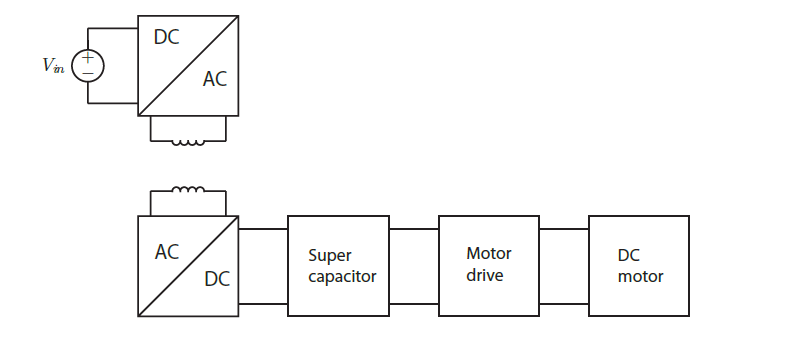
\includegraphics[width=0.8\linewidth]{resource/contactless_charging.png}
	\end{center}
	\caption{The wireless charging system with supercapacitors}
	\label{fig:contactless-charging}
\end{figure}

\section{Simulation}
We modelled the system by the circuit shown in Figure~\ref{fig:charg-circ}. $V_s$ denotes the source voltage, $C_1$ and $C_2$ the compensating capacitors, $R_1$ and $R_2$ the coil resistances, $L_1$ and $L_2$ the coil inductances, $M$ the mutual inductance and $R_L$ the load resistance. The coupling factor is defined by $k$.

\begin{figure}[H]
	\begin{center}
		\begin{circuitikz}[scale=1.2]
			 \draw (0,0) node[ground] {} to[american voltage source,l=$V_s$] (0,4)
				to[C, l=$C_1$] (2,4)
				to[european resistor, l=$R_1$] (4,4)
				to[L, l=$L_1$] (4,2);

			\draw (4,0) node[ground] {} to[american controlled voltage source, l=$j \omega M I_2$, i<=$I_1$] (4,2);

			\draw (6,0) node[ground] {} to[american controlled voltage source, l_=$j \omega M I_1$, i<=$I_2$] (6,2)
				to[L, l=$L_2$] (6,4)
				to[european resistor, l=$R_2$] (8,4)
				to[C, l=$C_2$] (10,4)
				to[european resistor, l=$R_L$] (10,0) node[ground] {};
		\end{circuitikz}
	\end{center}
	\caption{Equivalent circuit with compensation}
	\label{fig:charg-circ}
\end{figure}

Using the shown circuit, we derived the model

\begin{equation*}
	\mathbf{\vec{I}} \mathbf{Z}=
	\begin{bmatrix}
		I_{source} \\
		I_{load}
	\end{bmatrix}
	\begin{bmatrix}
		R_1 + j \omega L_1 + (j \omega C_1)^{-1}  & j \omega M\\
		j \omega M & R_2 + j \omega L_2 + (j \omega C_2)^{-1}  + R_L
	\end{bmatrix}
	= \mathbf{\vec{V}} =
	\begin{bmatrix}
		V_{source} \\
		0
	\end{bmatrix} .
\end{equation*}

This model translated to the transfer function

\begin{equation*}
	|H(s)| = \frac{s M Z_L}{(s M)^2 - (s L_2 + R_2 + (s C_2)^{-1} + Z_L) ( s L_1 + R1 + (s C_1)^{-1}))}
\end{equation*}

which is graphed in Figure~\ref{fig:charg-tf}.

\begin{figure}[H]
	\begin{center}
		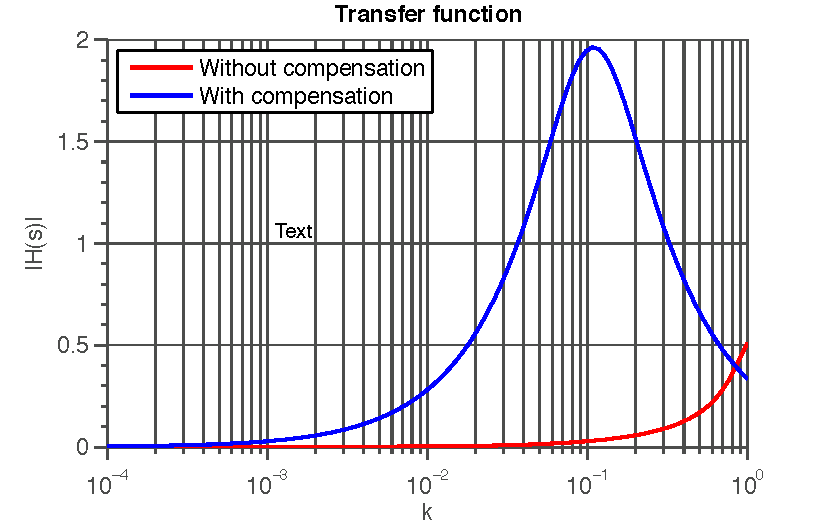
\includegraphics[width=0.8\linewidth]{resource/transfer-function.pdf}
	\end{center}
	\caption{Transfer function with and without compensation}
	\label{fig:charg-tf}
\end{figure}

We see that for a coupling factor of $k\approx0.1$ the power transferred is maximized. This corresponded with measurement results and a coil distance of approximately \SI{6}{cm}.

\section{System analysis}
To understand the way the power transfer is influenced by the distance between the coils, we have to go back to some elementary electromagnetics. When the distance increases, the coupling factor between both coils decreases. This causes the mutual inductance, and therefore the power transfer, to decrease. However, in the case of compensated coils, a decreased mutual inductance also causes an increased power drawn. There exists an optimal distance for which the resulting power transferred is maximized.

The DC/AC-inverter was made by making use of power electronics. For the coils' compensation to work, the generated signal's frequency had to match the resonance frequency. For this we used a frequency of \SI{100}{kHz}. For by trial-and-error optimized charging speed, we used a duty cycle of \num{0.4}. The parameters of the coils we used are displayed in Table~\ref{tab:charging-coil-params-calc}. The primary coil corresponds with the coil on the transmitting side, and the secondary coil with the coil on the receiving side.

\begin{table}[H]
	\centering
	\caption{Calculated coil parameters}
	\label{tab:charging-coil-params-calc}
	\begin{tabular}{c c c c c}
		\hline\hline
		Coil & Windings & Inductance & Outer diameter & Total wire length \\
		\hline
		Primary & \num{30} & \SI{101.6}{\micro H} & \SI{188}{mm} & \SI{11.2}{m} \\
		Secondary & \num{15} & \SI{22}{\micro H} & \SI{119}{mm} & \SI{4}{m} \\
		\hline
		\end{tabular}
\end{table} 

This system gave us a maximum charging speed of \num{3} minutes and \num{45} seconds and met all specified requirements.

\end{document}